%%%%%%%%%%%%%%%%%%%%%%%%%%%%%%%%%%%%%%%%%%%%%%%%%%%%%%%%%%%%
%%  This Beamer template was created by Cameron Bracken.
%%  Anyone can freely use or modify it for any purpose
%%  without attribution.
%%
%%  Last Modified: January 9, 2009
%%

\documentclass[xcolor=x11names,compress]{beamer}

%% General document %%%%%%%%%%%%%%%%%%%%%%%%%%%%%%%%%%
\usepackage{graphicx}
\usepackage{tikz}
\usetikzlibrary{decorations.fractals}
%%%%%%%%%%%%%%%%%%%%%%%%%%%%%%%%%%%%%%%%%%%%%%%%%%%%%%


%% Beamer Layout %%%%%%%%%%%%%%%%%%%%%%%%%%%%%%%%%%
\useoutertheme[subsection=false,shadow]{miniframes}
\useinnertheme{default}
\usefonttheme{serif}
\usepackage{palatino}
\usepackage{graphicx}
\usepackage{multicol}
\usepackage{amsmath}
\usepackage{epic,eepic,epsfig}
\usepackage{amssymb}
\usepackage{amstext}
\usetikzlibrary{shapes.geometric}

\usepackage{tikz}
\usepackage{mathtools}
\usetikzlibrary{arrows}
\usetikzlibrary{positioning}

\setbeamerfont{title like}{shape=\scshape}
\setbeamerfont{frametitle}{shape=\scshape}

\setbeamercolor*{lower separation line head}{bg=gray}%DeepSkyBlue4} 
\setbeamercolor*{normal text}{fg=black,bg=white} 
\setbeamercolor*{alerted text}{fg=red} 
\setbeamercolor*{example text}{fg=black} 
\setbeamercolor*{structure}{fg=black} 
 
\setbeamercolor*{palette tertiary}{fg=black,bg=black!10} 
\setbeamercolor*{palette quaternary}{fg=black,bg=black!10} 

\renewcommand{\(}{\begin{columns}}
\renewcommand{\)}{\end{columns}}
\newcommand{\<}[1]{\begin{column}{#1}}
\renewcommand{\>}{\end{column}}
\newcommand{\makepicture}{
\begin{figure}
\centering
  
\begin{tikzpicture}[scale=0.8,->,>=stealth',shorten >=1pt,auto,node distance=3cm,
    thick,main node/.style={circle,draw,font=\footnotesize}, small node/.style={circle,font=\footnotesize,inner sep=0pt,minimum size=5pt}]
   
   \begin{scope}
     
    \node[small node,fill=gray] (a) at (2,5) {};
    \node[small node,fill=gray] (b) at (4,5) {};
    \node[small node,fill=gray] (c) at (6,5) {};
    \node[small node,fill=gray] (d) at (8,5) {};
    \node[small node,fill=gray] (e) at (10,5) {};
    
    \path[-] (a) edge (b);
    \path[-] (b) edge (c);
    \path[-] (c) edge (d);
    \path[-] (d) edge (e);
    

   \end{scope}
  \end{tikzpicture} 
\end{figure}

}
%%%%%%%%%%%%%%%%%%%%%%%%%%%%%%%%%%%%%%%%%%%%%%%%%%




\begin{document}


%%%%%%%%%%%%%%%%%%%%%%%%%%%%%%%%%%%%%%%%%%%%%%%%%%%%%%
%%%%%%%%%%%%%%%%%%%%%%%%%%%%%%%%%%%%%%%%%%%%%%%%%%%%%%
\section{\scshape Introduction}
\begin{frame}
\title{How many oblivious robots can explore a line}
%\subtitle{SUBTITLE}
\author{
	Paola Flocchini  David Ilcinkas  Andrzej Pels  Nicola Santoro\\
	%{\it Humboldt State University}\\
	\vspace{24pt} 
	\includegraphics[width=1\textwidth,right]{robot1.jpg}
}
\titlepage
\end{frame}

%%%%%%%%%%%%%%%%%%%%%%%%%%%%%%%%%%%%%%%%%%%%%%%%%%%%%%
%%%%%%%%%%%%%%%%%%%%%%%%%%%%%%%%%%%%%%%%%%%%%%%%%%%%%%
% \begin{frame}{Introduction}
% \begin{multicols}{2}
% \tableofcontents
% \includegraphics[width=.4\textwidth,right]{robot1.jpg}
% \end{multicols}
% \end{frame}

%%%%%%%%%%%%%%%%%%%%%%%%%%%%%%%%%%%%%%%%%%%%%%%%%%%%%%
%%%%%%%%%%%%%%%%%%%%%%%%%%%%%%%%%%%%%%%%%%%%%%%%%%%%%%
\section{\scshape Model}
\subsection{frame 1}

\begin{frame}{}
\begin{tabular}{rl}
  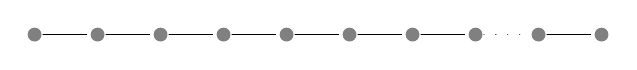
\begin{tikzpicture}[scale=0.8,->,>=stealth',shorten >=1pt,auto,node distance=3cm,
    thick,main node/.style={circle,draw,font=\footnotesize}, small node/.style={circle,font=\footnotesize,inner sep=0pt,minimum size=5pt}]   
    \begin{scope}     
%     \node[inner sep=0pt] (robot) at (4,5)
%     {\includegraphics[width=.02\textwidth,right]{robot1.jpg} };
      \node[small node,fill=gray] (a) at (1,5) {};
      \node[small node,fill=gray] (b) at (2,5) {};
      \node[small node,fill=gray] (c) at (3,5) {};
      \node[small node,fill=gray] (d) at (4,5) {};
      \node[small node,fill=gray] (e) at (5,5) {};    
      \node[small node,fill=gray] (f) at (6,5) {};
      \node[small node,fill=gray] (g) at (7,5) {};
      \node[small node,fill=gray] (h) at (8,5) {};
      \node[small node,fill=gray] (i) at (9,5) {};
      \node[small node,fill=gray] (j) at (10,5) {}; 
      \path[-,line width=0.3pt] (a) edge (b);
      \path[-,line width=0.3pt] (b) edge (c);
      \path[-,line width=0.3pt] (c) edge (d);
      \path[-,line width=0.3pt] (d) edge (e);
      \path[-,line width=0.3pt] (e) edge (f);
      \path[-,line width=0.3pt] (f) edge (g);
      \path[-,line width=0.3pt] (g) edge (h);
      \path[-,line width=0.3pt, loosely dotted] (h) edge (i);
      \path[-,line width=0.3pt] (i) edge (j);
    \end{scope}
  \end{tikzpicture} 
  & $n$ nodes\\ 
      &  \\
  \includegraphics[width=.05\textwidth,right]{robot1.jpg} 
  \includegraphics[width=.05\textwidth,right]{robot1.jpg} 
  \includegraphics[width=.05\textwidth,right]{robot1.jpg}  
  \includegraphics[width=.05\textwidth,right]{robot1.jpg} 
  & $k$ robots\\
    &  \\
        &  \\
    \begin{tikzpicture}[scale=0.8,->,>=stealth',shorten >=1pt,auto,node distance=3cm,
    thick,main node/.style={circle,draw,font=\footnotesize}, small node/.style={circle,font=\footnotesize,inner sep=0pt,minimum size=5pt}]   
    \begin{scope}     
%     \node[inner sep=0pt] (robot) at (4,5)
%     {\includegraphics[width=.02\textwidth,right]{robot1.jpg} };
      \node[small node,fill=gray] (a) at (1,5) {};
      \node[inner sep=0pt]  (b) at (2,5) {\includegraphics[width=.03\textwidth,right]{robot1.jpg}};
      \node[small node,fill=gray] (c) at (3,5) {};
      \node[inner sep=0pt]  (d) at (4,5) {\includegraphics[width=.03\textwidth,right]{robot1.jpg}};
      \node[inner sep=0pt]  (e) at (5,5) {\includegraphics[width=.03\textwidth,right]{robot1.jpg}};    
      \node[small node,fill=gray] (f) at (6,5) {};
      \node[inner sep=0pt]  (g) at (7,5) {\includegraphics[width=.03\textwidth,right]{robot1.jpg}};
      \node[small node,fill=gray] (h) at (8,5) {};
      \node[small node,fill=gray] (i) at (9,5) {};
      \node[small node,fill=gray] (j) at (10,5) {}; 
      
%       \node[inner sep=0pt]   at (2,5.5) {\includegraphics[width=.03\textwidth,right]{robot1.jpg}};
%       \node[inner sep=0pt]   at (5,5.5) {\includegraphics[width=.03\textwidth,right]{robot1.jpg}};
%       \node[inner sep=0pt]   at (5,6) {\includegraphics[width=.03\textwidth,right]{robot1.jpg}};
      \path[-,line width=0.3pt] (a) edge (b);
      \path[-,line width=0.3pt] (b) edge (c);
      \path[-,line width=0.3pt] (c) edge (d);
      \path[-,line width=0.3pt] (d) edge (e);
      \path[-,line width=0.3pt] (e) edge (f);
      \path[-,line width=0.3pt] (f) edge (g);
      \path[-,line width=0.3pt] (g) edge (h);
      \path[-,line width=0.3pt, loosely dotted] (h) edge (i);
      \path[-,line width=0.3pt] (i) edge (j);
    \end{scope}
  \end{tikzpicture}
  & \\
\end{tabular}
\end{frame}

\begin{frame}{Look}

%\resizebox{<horizontal size>}{<vertical size>}{%
    \begin{tikzpicture}[scale=0.8,->,>=stealth',shorten >=1pt,auto,node distance=3cm,
    thick,main node/.style={circle,draw,font=\footnotesize}, small node/.style={circle,font=\footnotesize,inner sep=0pt,minimum size=5pt}]   

    \begin{scope}%[xshift=10cm]
      \node[small node,fill=gray] (b) at (2,5) {};
      \node[inner sep=0pt]  (c) at (4,5) {\includegraphics[width=.03\textwidth,right]{robot1.jpg}};
      \node[inner sep=0pt]  (d) at (6,5) {\includegraphics[width=.03\textwidth,right]{robot1.jpg}};
      \node[small node,fill=gray] (e) at (8,5) {};    
      \node[inner sep=0pt]  (f) at (10,5) {\includegraphics[width=.03\textwidth,right]{robot1.jpg}};
      \node[inner sep=0pt] at (10,5.5) {\includegraphics[width=.03\textwidth,right]{robot1.jpg}};
      \node[small node,fill=gray] (i) at (12,5) {};
      \node[small node,fill=gray] (j) at (14,5) {};
      \path[-,line width=0.3pt] (b) edge (c);
      \path[-,line width=0.3pt] (c) edge (d);
      \path[-,line width=0.3pt] (d) edge (e);
      \path[-,line width=0.3pt] (e) edge (f);
      \path[-,line width=0.3pt, loosely dotted] (f) edge (i);
      \path[-,line width=0.3pt] (i) edge (j);

      \path[-,line width=0.3pt, color=pink] (d) edge [bend right,-] (7.2,6.8);
% 
%       
    \end{scope}
        \begin{scope}[scale=0.4, xshift=12cm,yshift=12cm]
      \node[small node,fill=gray] (b) at (2,5) {};
      \node[small node,fill=gray] (c) at (4,5) {};
      %\node[inner sep=0pt]  (d) at (6,5) {\includegraphics[width=.03\textwidth,right]{robot1.jpg}};
      \node[small node,fill=pink] (d) at (6,5) {};
      \node[small node,fill=gray] (e) at (8,5) {};    
      \node[small node,fill=gray] (f) at (10,5) {};
      \node[small node,fill=gray] (i) at (12,5) {};
      \node[small node,fill=gray] (j) at (14,5) {};
      \path[-,line width=0.3pt] (b) edge (c);
      \path[-,line width=0.3pt] (c) edge (d);
      \path[-,line width=0.3pt] (d) edge (e);
      \path[-,line width=0.3pt] (e) edge (f);
      \path[-,line width=0.3pt, loosely dotted] (f) edge (i);
      \path[-,line width=0.3pt] (i) edge (j);
    \end{scope}
  \end{tikzpicture}
\end{frame}


\begin{frame}{Look}

%\resizebox{<horizontal size>}{<vertical size>}{%
    \begin{tikzpicture}[scale=0.8,->,>=stealth',shorten >=1pt,auto,node distance=3cm,
    thick,main node/.style={circle,draw,font=\footnotesize}, small node/.style={circle,font=\footnotesize,inner sep=0pt,minimum size=5pt}]   

    \begin{scope}%[xshift=10cm]
      \node[small node,fill=gray] (b) at (2,5) {};
      \node[inner sep=0pt]  (c) at (4,5) {\includegraphics[width=.03\textwidth,right]{robot1.jpg}};
      \node[inner sep=0pt]  (d) at (6,5) {\includegraphics[width=.03\textwidth,right]{robot1.jpg}};
      \node[small node,fill=gray] (e) at (8,5) {};    
      \node[inner sep=0pt]  (f) at (10,5) {\includegraphics[width=.03\textwidth,right]{robot1.jpg}};
      \node[inner sep=0pt] at (10,5.5) {\includegraphics[width=.03\textwidth,right]{robot1.jpg}};
      \node[small node,fill=gray] (i) at (12,5) {};
      \node[small node,fill=gray] (j) at (14,5) {};
      \path[-,line width=0.3pt] (b) edge (c);
      \path[-,line width=0.3pt] (c) edge (d);
      \path[-,line width=0.3pt] (d) edge (e);
      \path[-,line width=0.3pt] (e) edge (f);
      \path[-,line width=0.3pt, loosely dotted] (f) edge (i);
      \path[-,line width=0.3pt] (i) edge (j);

      \path[-,line width=0.3pt, color=pink] (d) edge [bend right,-] (7.2,6.8);
% 
%       
    \end{scope}
        \begin{scope}[scale=0.4, xshift=12cm,yshift=12cm]
      \node[small node,fill=gray] (b) at (2,5) {};
      \node[small node,fill=black] (c) at (4,5) {};
      %\node[inner sep=0pt]  (d) at (6,5) {\includegraphics[width=.03\textwidth,right]{robot1.jpg}};
      \node[small node,fill=pink] (d) at (6,5) {};
      \node[small node,fill=gray] (e) at (8,5) {};    
      \node[diamond, fill=black]  (f) at (10,5) {};
      \node[small node,fill=gray] (i) at (12,5) {};
      \node[small node,fill=gray] (j) at (14,5) {};
      \path[-,line width=0.3pt] (b) edge (c);
      \path[-,line width=0.3pt] (c) edge (d);
      \path[-,line width=0.3pt] (d) edge (e);
      \path[-,line width=0.3pt] (e) edge (f);
      \path[-,line width=0.3pt, loosely dotted] (f) edge (i);
      \path[-,line width=0.3pt] (i) edge (j);

    \end{scope}
  \end{tikzpicture}
\end{frame}



\begin{frame}{Look}

%\resizebox{<horizontal size>}{<vertical size>}{%
    \begin{tikzpicture}[scale=0.8,->,>=stealth',shorten >=1pt,auto,node distance=3cm,
    thick,main node/.style={circle,draw,font=\footnotesize}, small node/.style={circle,font=\footnotesize,inner sep=0pt,minimum size=5pt}]   

    \begin{scope}%[xshift=10cm]
      \node[small node,fill=gray] (b) at (2,5) {};
      \node[inner sep=0pt]  (c) at (4,5) {\includegraphics[width=.03\textwidth,right]{robot1.jpg}};
      \node[inner sep=0pt]  (d) at (6,5) {\includegraphics[width=.03\textwidth,right]{robot1.jpg}};
      \node[small node,fill=gray] (e) at (8,5) {};    
      \node[inner sep=0pt]  (f) at (10,5) {\includegraphics[width=.03\textwidth,right]{robot1.jpg}};
      \node[inner sep=0pt] at (10,5.5) {\includegraphics[width=.03\textwidth,right]{robot1.jpg}};
      \node[small node,fill=gray] (i) at (12,5) {};
      \node[small node,fill=gray] (j) at (14,5) {};
      \path[-,line width=0.3pt] (b) edge (c);
      \path[-,line width=0.3pt] (c) edge (d);
      \path[-,line width=0.3pt] (d) edge (e);
      \path[-,line width=0.3pt] (e) edge (f);
      \path[-,line width=0.3pt, loosely dotted] (f) edge (i);
      \path[-,line width=0.3pt] (i) edge (j);

      \path[-,line width=0.3pt, color=pink] (f) edge [bend right,-] (7.2,6.8);
% 
%       
    \end{scope}
        \begin{scope}[scale=0.4, xshift=12cm,yshift=12cm]
      \node[small node,fill=gray] (b) at (2,5) {};
      \node[small node,fill=black] (c) at (4,5) {};
      %\node[inner sep=0pt]  (d) at (6,5) {\includegraphics[width=.03\textwidth,right]{robot1.jpg}};
      \node[small node,fill=black] (d) at (6,5) {};
      \node[small node,fill=gray] (e) at (8,5) {};    
      \node[diamond, fill=pink]  (f) at (10,5) {};
      \node[small node,fill=gray] (i) at (12,5) {};
      \node[small node,fill=gray] (j) at (14,5) {};
      \path[-,line width=0.3pt] (b) edge (c);
      \path[-,line width=0.3pt] (c) edge (d);
      \path[-,line width=0.3pt] (d) edge (e);
      \path[-,line width=0.3pt] (e) edge (f);
      \path[-,line width=0.3pt, loosely dotted] (f) edge (i);
      \path[-,line width=0.3pt] (i) edge (j);

    \end{scope}
  \end{tikzpicture}
\end{frame}

% \begin{itemize}
% \item Item A
% \item Item B
% \begin{itemize}
% \item Subitem 1
% \item Subtem 2
% \end{itemize}
% \item Item C
% \end{itemize}
%%%%%%%%%%%%%%%%%%%%%%%%%%%%%%%%%%%%%%%%%%%%%%%%%%%%%%
%%%%%%%%%%%%%%%%%%%%%%%%%%%%%%%%%%%%%%%%%%%%%%%%%%%%%%
\subsection{frame 2}
\begin{frame}{frame 2}
\begin{multicols}{3}
% [
% %\section{First Section}
% All human things are subject to decay. And when fate summons, Monarchs must obey.
% ]
Hello, here is some text without a meaning.  This text should show what 
a printed text will look like at this place.
If you read this text, you will get no information.  Really?  Is there 
no information?  Is there...
\end{multicols}
\end{frame}

%%%%%%%%%%%%%%%%%%%%%%%%%%%%%%%%%%%%%%%%%%%%%%%%%%%%%%
%%%%%%%%%%%%%%%%%%%%%%%%%%%%%%%%%%%%%%%%%%%%%%%%%%%%%%
\subsection{frame 3}
\begin{frame}{frame 3}

\end{frame}


%%%%%%%%%%%%%%%%%%%%%%%%%%%%%%%%%%%%%%%%%%%%%%%%%%%%%%
%%%%%%%%%%%%%%%%%%%%%%%%%%%%%%%%%%%%%%%%%%%%%%%%%%%%%%
\section{\scshape Methodology}
\subsection{frame 1}
\begin{frame}{frame 1}

\end{frame}


%%%%%%%%%%%%%%%%%%%%%%%%%%%%%%%%%%%%%%%%%%%%%%%%%%%%%%
%%%%%%%%%%%%%%%%%%%%%%%%%%%%%%%%%%%%%%%%%%%%%%%%%%%%%%
\subsection{frame 1}
\begin{frame}{frame 1}

\end{frame}

%%%%%%%%%%%%%%%%%%%%%%%%%%%%%%%%%%%%%%%%%%%%%%%%%%%%%%
%%%%%%%%%%%%%%%%%%%%%%%%%%%%%%%%%%%%%%%%%%%%%%%%%%%%%%
\section{\scshape Results}
\subsection{Frame 1}
\begin{frame}{Frame 1}



\begin{figure}
\centering
  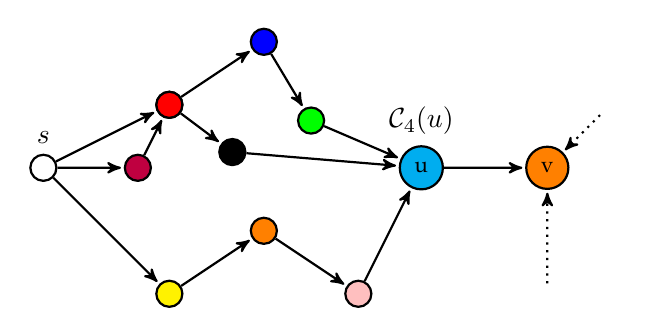
\begin{tikzpicture}[scale=0.8,->,>=stealth',shorten >=1pt,auto,node distance=3cm,
    thick,main node/.style={circle,draw,font=\footnotesize}]
   
   \begin{scope}[shift={(-10,0)}]
    
    \node[main node, label=above:$s$] (s) at (0,5) {};
    
    \node[main node, label=above:$\mathcal{C}_4(u)$, fill=cyan] (u) at (6,5) {u};
    \node[main node, fill=orange] (v) at (8,5) {v};
    \draw (u)-- (v);
    
    
    \node[main node,fill=red] (b) at (2,6) {};
    \node[main node,fill=blue] (f) at (3.5,7) {};
    \node[main node,fill=green] (g) at (4.25,5.75) {};
    \draw (s)--(b);
    \draw (b)--(f);
    \draw (f)--(g);
    \draw (g)--(u);
    
    \node[main node,fill=purple] (b) at (1.5,5) {};
    \node[main node, fill=red] (f) at (2,6) {};
    \node[main node, fill=black] (g) at (3,5.25) {};
    \draw (s)--(b);
    \draw (b)--(f);
    \draw (f)--(g);
    \draw (g)--(u);
    
    
    \node[main node, fill=yellow] (b) at (2,3) {};
    \node[main node, fill=orange] (f) at (3.5,4) {};
    \node[main node, fill=pink] (g) at (5,3) {};
    \draw (s)--(b);
    \draw (b)--(f);
    \draw (f)--(g);
    \draw (g)--(u);
    
    
    \node[] (p) at (8,3) {};
    \node[] (q) at (9,6) {};
    \draw[dotted] (p) -- (v);
    \draw[dotted] (q) -- (v);
   \end{scope}
  \end{tikzpicture} 
  \caption{Figure illustrating the dynamic programming. On left for $i=4$ $\mathcal{C}_4(u) = \{ \{\text{ red, blue, green, cyan}\}, \{\text{purple, red, black, cyan}\}, \{\text{yellow, orange, pink, cyan}\} \}$. On the right for $i=5$ $\mathcal{C}_5(v) = \{ \{\text{red, blue, green, cyan,orange}\}, \{\text{purple, red, black, cyan,orange}\}\}$. Notice that the set from $\mathcal{C}_4(u)$ with the color orange are not used in $\mathcal{C}_5(v)$ as $c(v)$ is orange. }\label{FigColoring}
\end{figure}


\end{frame}

\end{document}